\documentclass[10pt]{article}
\usepackage{graphicx}
\graphicspath{ {./} }

\title{UML Assignment 3}

\author{Himanshu Patel (C0735691), Shubham (C0737342), Sujalkumar Patel (C0735603)\\Jattinder Kaur (C0737459), Palwinder Kaur (C0737690), Navneet Kaur (C07354154)}

\date{5 July, 2019}

\begin{document}
\maketitle
\tableofcontents

\newpage
\section{Use Case - Develop Project Time Management Plan}
\subsection{Goal- To Enable Project Manager to Develop Project Time Management Plan}
\subsection{Actors - Project Manager, Team Members}
\subsection{Scenario}
\begin{itemize}
  \item Provide GUI for Project Manager to Define Activities by identifying and documenting the specific actions to be performed to produce the project deliverables.
  \item Provide GUI for Project Manager to Sequence Activities by identifying and documenting relationships among the project activities.
  \item Provide GUI for Project Manager to Estimate Activity Resources by estimating the type and quantities of material, human resources, equipment, or supplies required to perform each activity.
  \item Provide GUI for Project Manager to Estimate Activity Durations by estimating the number of work periods needed to complete individual activities with estimated resources.
  \item Provide GUI for Project Manager to Develop Schedule by analyzing activity sequences, durations, resource requirements, and schedule constraints to create the project schedule model.
  \item download the document as a pdf by selecting Export $>$ Local
        Filesystem (or by clicking the desktop download button)
  \item Provide GUI for Project Manager to Control Schedule by monitoring the status of project activities to update project progress and manage changes to the schedule baseline to achieve the plan.
\end{itemize}

\subsection{UML}
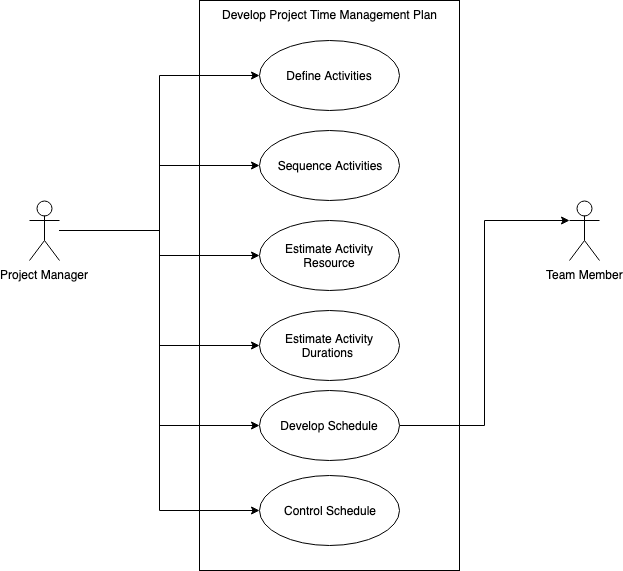
\includegraphics[width=\textwidth]{usecase1}

\newpage
\section{Use Case - Develop Project Cost Management Plan}
\subsection{Goal- To Enable Project Manager to Develop Project Cost Management Plan}
\subsection{Actors - Project Manager, Stake Holders}
\subsection{Scenario}
\begin{itemize}
  \item Provide GUI for Project Manager to Estimate Costs by developing an approximation of the monetary resources needed to complete project activities.
  \item Provide GUI for Project Manager to Determine Budget by aggregating the estimated costs of individual activities or work packages to establish an authorized cost baseline.
  \item Provide GUI for Project Manager to Control Costs by monitoring the status of the project to update the project costs and managing changes to the cost baseline.
  
\end{itemize}

\subsection{UML}
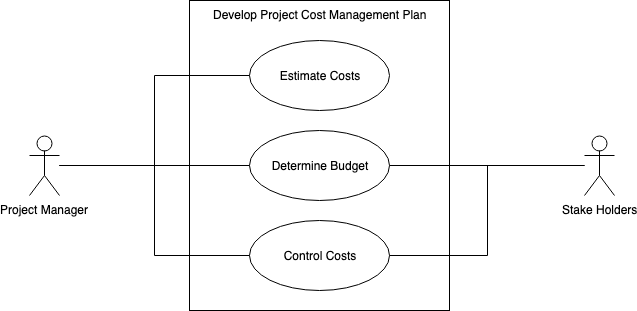
\includegraphics[width=\textwidth]{usecase2}

\newpage
\section{Use Case - Develop Project Quality Management Plan}
\subsection{Goal- To Enable Project Manager to Develop Project Quality Management Plan}
\subsection{Actors - Project Manager, Quality Analyst, Team Members}
\subsection{Scenario}
\begin{itemize}
  \item Provide GUI to Plan Quality Management by identifying quality requirements and standards for the project and its deliverables and documenting how the project will demonstrate compliance with quality requirements.
  \item Provide GUI to Perform Quality Assurance by auditing the quality requirements and the results from quality control measurements to ensure that appropriate quality standards and operational definitions are used.
  \item Provide GUI to Control Quality by monitoring and recording results of executing the quality activities to assess performance and recommend necessary changes.
  
\end{itemize}

\subsection{UML}
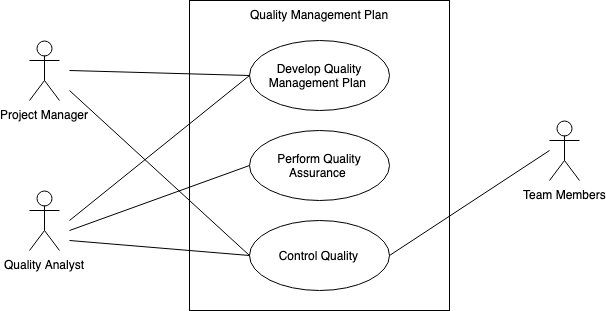
\includegraphics[width=\textwidth]{usecase3}

\end{document}
